\section[Проектирование программного модуля]{%
  ПРОЕКТИРОВАНИЕ ПРОГРАММНОГО МОДУЛЯ
}\label{sec:design}

\subsection{Общая характеристика задачи}

Проектирование является неотъемлемой частью жизненного цикла
разработки программного обеспечения.
Существует множество различных методологий проектирования.
Каждая из них предполагает описание требований к разрабатываемой системе
и собственно разработку структуры системы, которая им удовлетворяет.
В ходе проектирования требования к системе многократно дополняются и уточняются.
Характер процесса проектирования определятся используемой
методологией разработки программного обеспечения.
Существует две основные методологии разработки ПО:
каскадная и итеративная, представленные на рисунке~\ref{fig:design_methods}.

\begin{figure}[h!]
  \centering
  \fcolorbox{gray}{white}{
    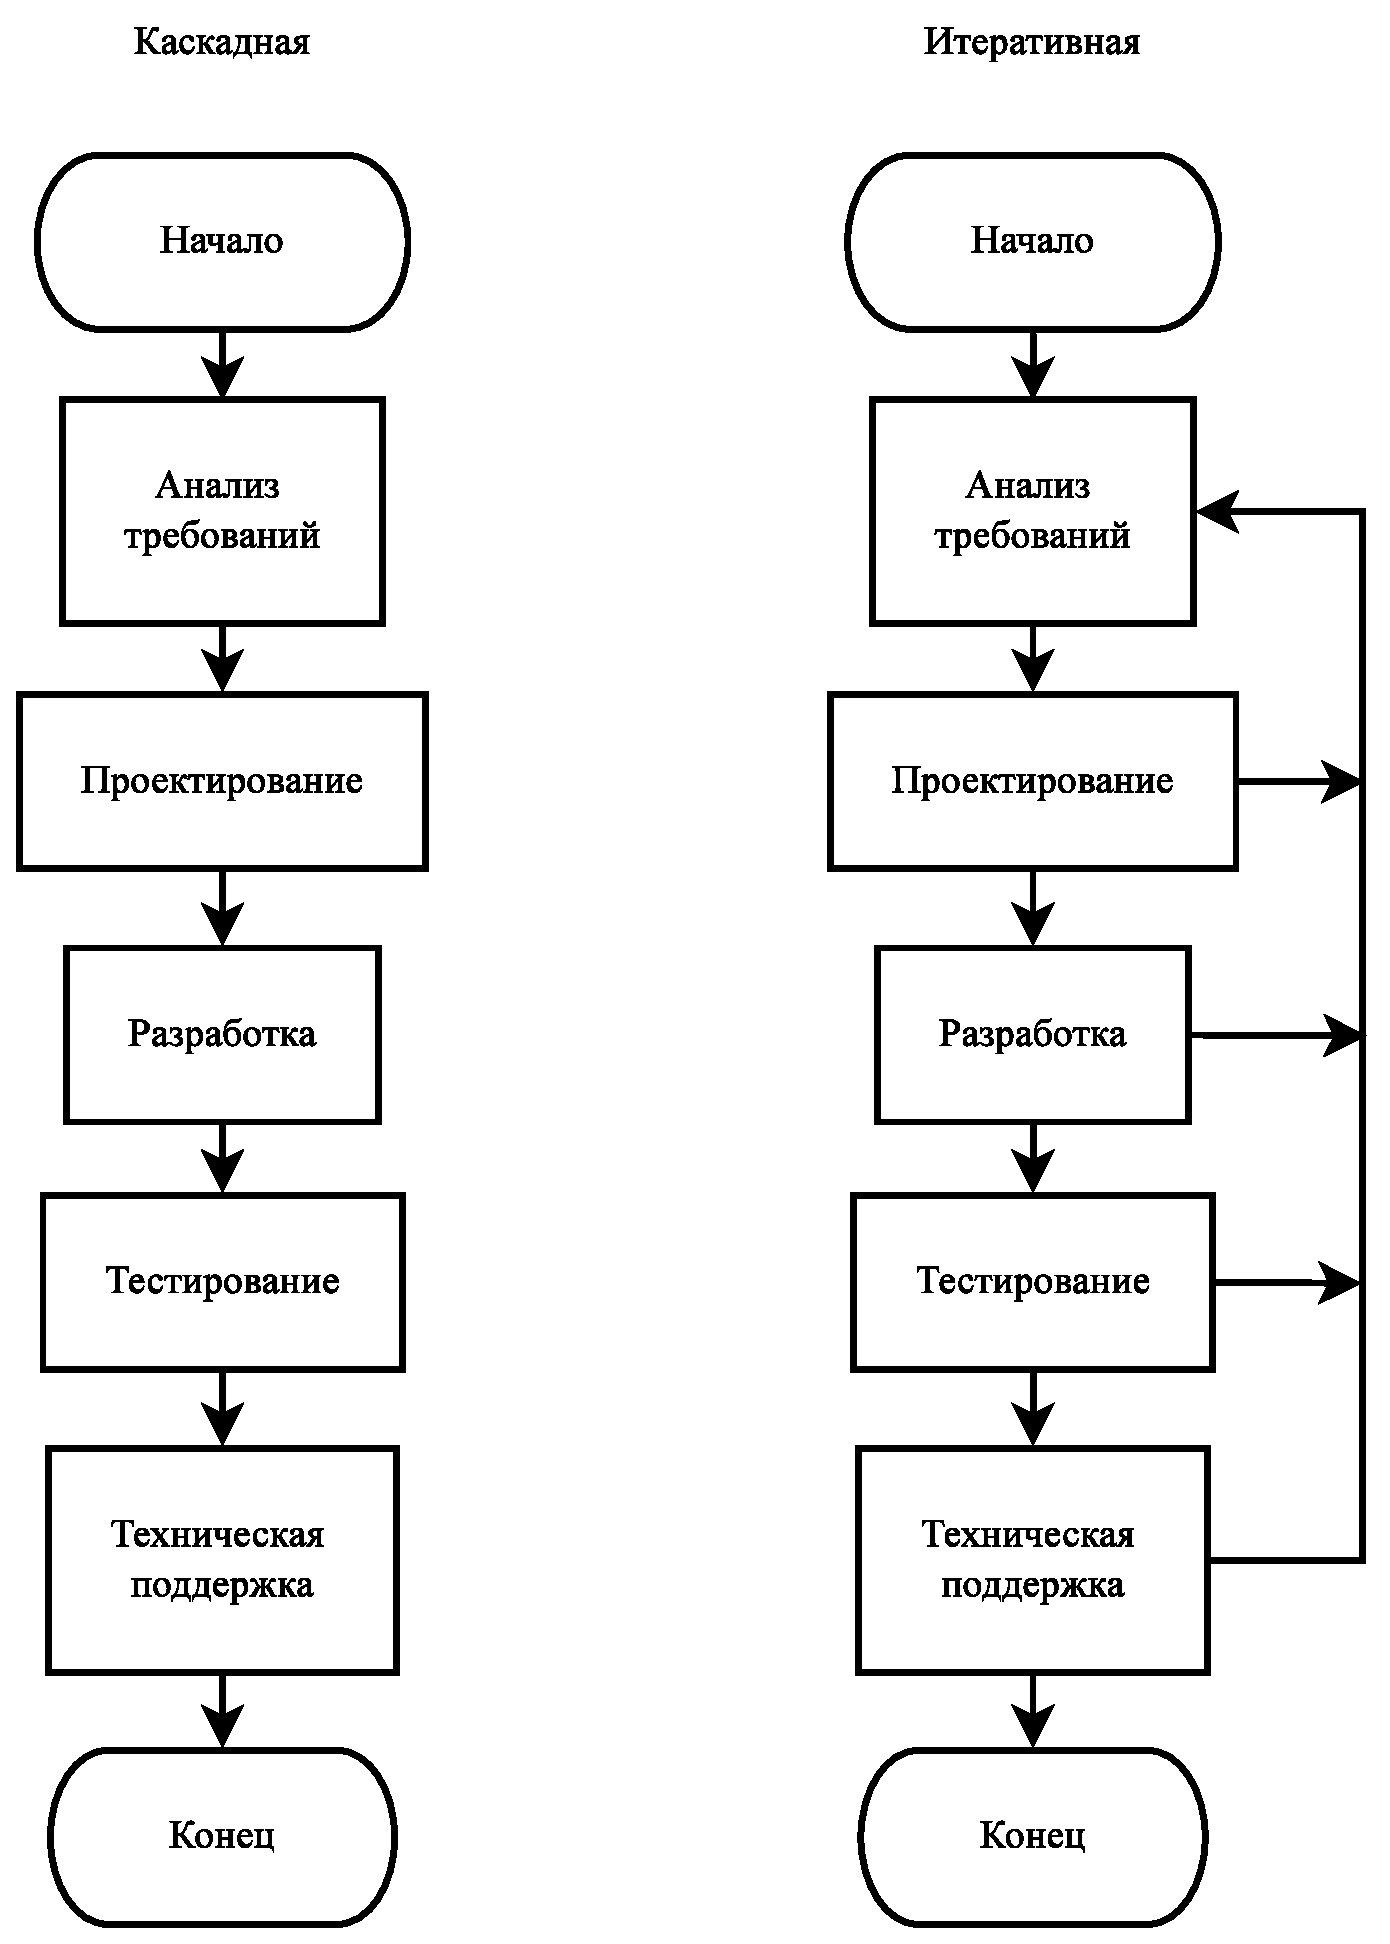
\includegraphics[width=90mm]{fig/design_methods.eps}
  }
  \caption{Методологии разработки \\ программного обеспечения}
  \label{fig:design_methods}
\end{figure}

Каскадная методология разработки ПО сводится к последовательному
прохождению набора фаз разработки:
анализа требований, проектирования, реализации, тестирования, интеграции и поддержки.
При использовании данной методологии проектирование производится
лишь один раз. Входными данными являются требования к продукту,
а результатом --- набор технических документов, детально описывающих
разрабатываемую систему.
Дальнейшие этапы разработки производятся в строгом соответствии с этими документами;
изменение их содержания на последующих этапах не приветствуется.

Итеративная методология рассматривает процесс разработки ПО как
циклическое прохождение описанных выше фаз разработки.
Это позволяет команде разработчиков динамичнее реагировать
как на внутренние, так и на внешние изменения требований к продукту разработки.
При использовании данной методологии проектирование производится несколько раз.
На первых порах разрабатывается высокоуровневая архитектура системы,
определяются ключевые требования к ней. Далее, по мере повторения цикла
разработки, производится описание разрабатываемых подсистем и связей между ними.

Данный проект разрабатывается с использованием итеративной методологии:
сначала будет выполняется высокоуровневое описание частей проекта,
а затем по мере реализации уточняются детали функционирования его подсистем.
Проектирование выполняется с использованием языка графического
моделирования UML~\cite{fowler04}, а также набора документированных решений,
известных как паттерны проектирования GoF~\cite{gamma01}.

Объектом проектирования является мобильное приложение,
которое представляет собой самостоятельный программный модуль.
Поскольку необходимость интеграции в какую-либо существующую
систему отсутствует, задача проектирования значительно упрощается.
С другой стороны, целевая мобильная платформа выдвигает ряд дополнительных
требований к объекту проектирования:
\begin{itemize}
\item более строгие ограничения на используемые ресурсы;
\item учет разнообразия конфигураций мобильных устройств;
\item поддержка совместимости между различными версиями
  мобильной платформы.
\end{itemize}

Мобильные устройства располагают, как правило, меньшими вычислительными
ресурсами по сравнению с ПК. Кроме этого, при разработке приложения для
мобильной платформы требуется учитывать его влияние на энергопотребление.
Размер и плотность дисплеев мобильных устройств изменяется в широких пределах,
что влияет на качество отображения информации, предоставляемой приложением.
Программные интерфейсы различных версий мобильной платформы
могут быть несовместимы между собой.

Объектом проектирования является мобильное приложение,
выполняющее учет финансовых данных. По большому счету, пользователь
ожидает от него выполнения двух основных функций:
ввода финансовых данных и представления статистики на основе этих данных,
как показано на рисунке~\ref{fig:design_use_cases}.

\begin{figure}[h!]
  \centering
  \fcolorbox{gray}{white}{
    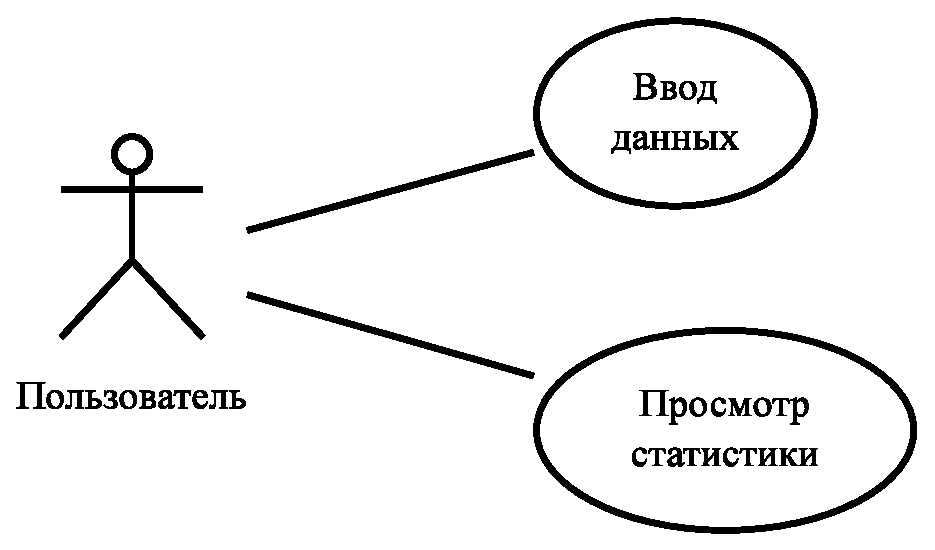
\includegraphics[width=90mm]{fig/design_use_cases.eps}
  }
  \caption{Диаграмма прецендентов \\ использования приложения}
  \label{fig:design_use_cases}
\end{figure}

В нашем случае основную важность имеет не столько богатство
функциональности приложения, сколько удобство его повседневного использования.
В связи с этим на первый план выходят такие требования, как
высокая скорость ввода данных и наглядность их представления.
Скорость ввода данных достигается в первую очередь за счет
продуманного интерфейса приложения ---
ввод данных должен требовать заполнения минимально числа полей;
интерфейс ввода должен быть как можно более простым.
Наглядность представления данных достигается за счет надлежащей
структуризации данных и использования визуальных средств представления.
Поскольку приложение выполняет хранение данных, возникает необходимость
разработки модели данных и использовании соответствующей базы данных.
Кроме этого, для реализации функции ввода данных с изображения
также требуется разработать соответствующую подсистему.

\subsection{Структура разрабатываемого модуля}
\label{subsec:design_structure}

Фундаментальной проблемой, возникающей при разработке программного обеспечения,
является проблема управления сложностью. Зачастую моделируемые объекты реального
мира и механизмы их взаимодействия являются чересчур сложными для восприятия человека.
Дополнительную сложность вносят детали программной
реализации, которые радикально отличаются от сущности объекта моделирования.

Основным средством борьбы со сложностью при разработке программного обеспечения
на данным момент можно считать объектно-ориентированный подход.
Этот подход вводит понятие объекта как базового элемента
архитектуры системы, а также понятие абстракции как средства
разбиения проектируемой системы на логические уровни.
Модели, полученные с использованием данного подхода, весьма точно
описывают предметную область и являются сравнительно простыми для понимания.

В ходе практики использования объектно-ориентированного подхода
был разработан набор полезных <<рецептов>>,
позволяющих решать некоторые типичные проблемы проектирования.
Данные <<рецепты>>, называемые паттернами проектирования,
описывают различные механизмы создания, структуризации и взаимодействия объектов.

Паттерны проектирования особенно часто используются при разработке
библиотек и фреймворков.
Библиотеки представляют собой наборы структур данных и
связанных с ними алгоритмов для решения задач определенного класса,
например, ввод/вывод данных, рисование графиков, тестирование, и~т.~д.
Фреймворки представляют собой типовые программные решения
типичных задач программирования.
В отличие от библиотек, фреймворки определяют структуру приложения в целом,
позволяя при этом разработчикам добавлять желаемые функции путем
добавления нового программного кода, а также переопределения
части программного кода своих компонентов.

Разработка приложения для платформы Android предполагает использование
объектно-ориентированного подхода. Несмотря на то, что в общем случае
платформа не предписывает использования какого-либо фреймворка,
ее программный интерфейс накладывает существенные ограничения на
архитектуру приложения.
Поскольку разрабатываемое приложение имеет графический интерфейс,
имеет смысл выполнять его проектирование на базе паттернов
разработки приложений с графическим интерфейсом.
Примером одного из них является MVP --- model-view-presenter,
представленный на рисунке~\ref{fig:design_mvp}.

\begin{figure}[h!]
  \centering
  \fcolorbox{gray}{white}{
    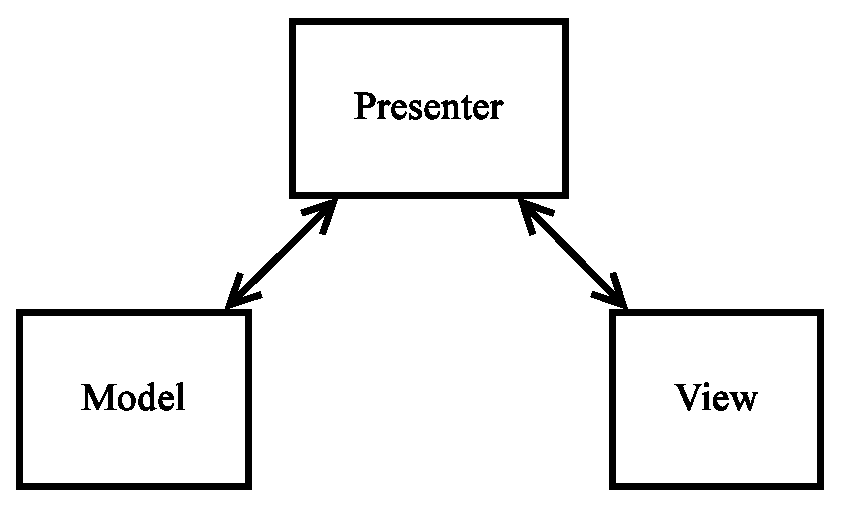
\includegraphics[width=82mm]{fig/design_mvp.eps}
  }
  \caption{Паттерн проектирования MVP}
  \label{fig:design_mvp}
\end{figure}

Основной идеей данного паттерна является разделение объектов приложения на три типа.
Объекты типа Model представляют собой ресурсы приложения, как они организуют доступ
к базе данных. Объекты типа View занимаются представлением данных. Они определяют,
в каком виде данные будут показываться пользователю. Взаимодействие этих объектов
производится через объекты типа Presenter, определяющих логику
обработки данных (бизнес-логику). В этом заключается основное отличие данного паттерна от
его предшественника MVC.
На рисунке~\ref{fig:design_main} представлена структура проектируемого приложения.

\begin{figure}[h!]
  \centering
  \fcolorbox{gray}{white}{
    \includegraphics[width=140mm]{fig/design_main.eps}
  }
  \caption{Структура приложения}
  \label{fig:design_main}
\end{figure}

Здесь Model соответствуют подсистемам хранения данных и компьютерного зрения;
Presenter --- обработки данных, а View --- графического интерфейса.
Как и предписывается паттерном MVP, подсистемы графического интерфейса,
базы данных и компьютерного зрения изолированы друг от друга и взаимодействуют
между собой через слой обработки данных.

Рассмотрим структуру пользовательского интерфейса более подробно.
Пользовательский интерфейс приложений для платформы Android состоит
из так называемых экранов.
Экран по сути соответствует окну оконного менеджера графической оболочки
операционной системы. Основное отличие заключается в том, что
экраны не могут перекрываться, т.~е. экран занимает все пространство дисплея
мобильного устройства.
Как правило, каждый экран приложения предназначен
для выполнения какой-либо одной функции.
На рисунке~\ref{fig:design_activities} представлена схема экранов приложения
и переходов между ними.

\begin{figure}[h!]
  \centering
  \fcolorbox{gray}{white}{
    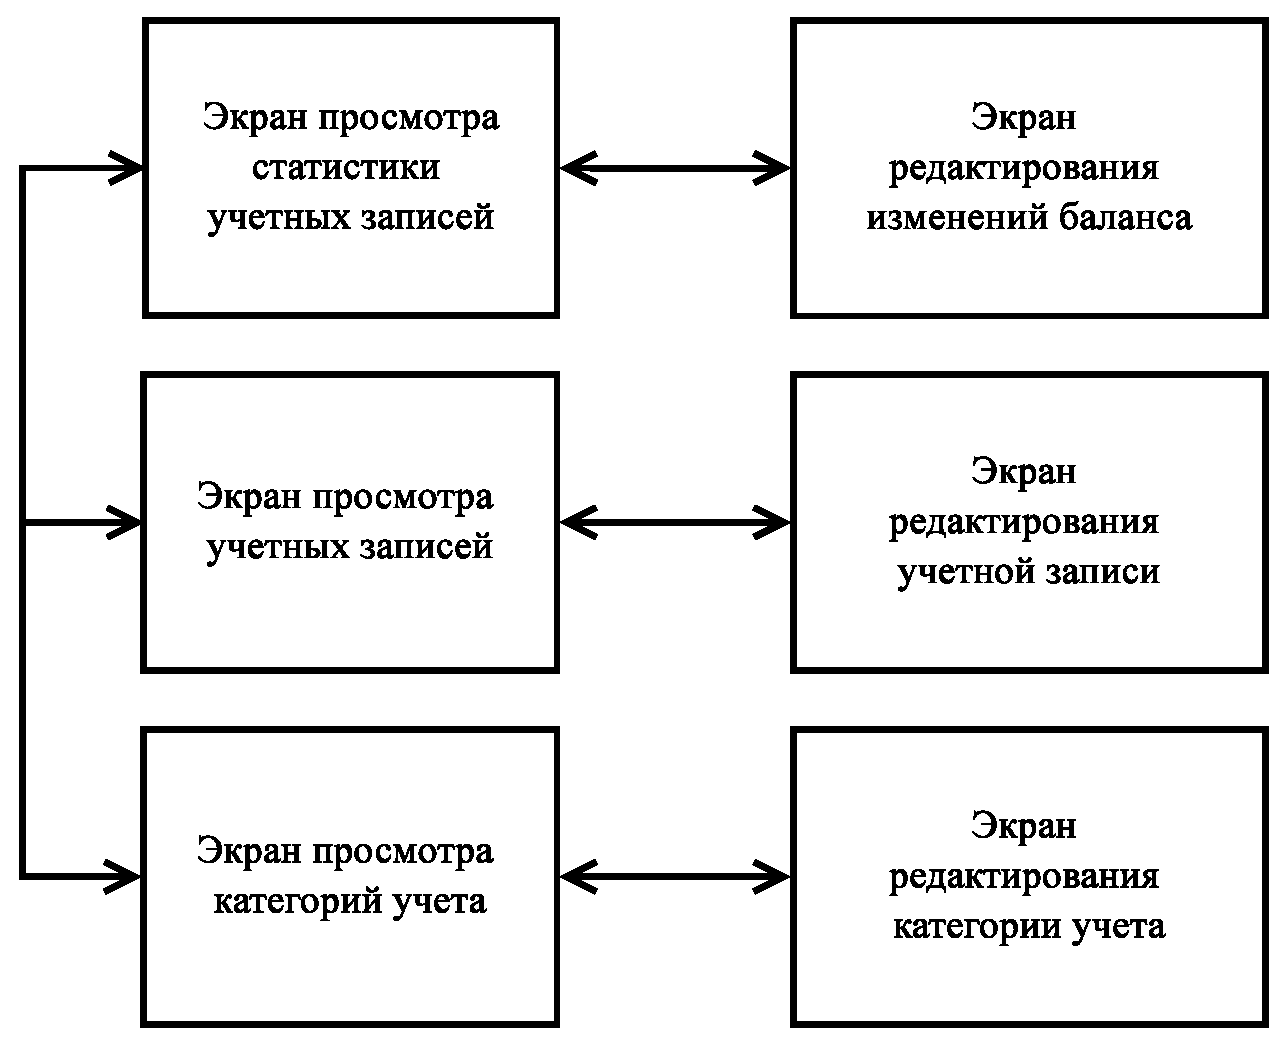
\includegraphics[width=130mm]{fig/design_activities.eps}
  }
  \caption{Схема экранов приложения}
  \label{fig:design_activities}
\end{figure}

Приложение состоит из семи экранов, возможные переходы между экранами
показаны стрелками. Выполним краткое описание каждого экрана приложения.
Экран просмотра статистики учетных записей является главным экраном приложения
и предназначен для отображения информации об учетных записях пользователя,
а также списка изменений состояния баланса.
Экраны редактирования изменений баланса, учетных записей и категорий
используются для добавления и изменения выбранного изменения баланса,
учетной записи и категории соответственно.
Экраны просмотра списков учетных записей и категорий используются
для просмотра и удаления учетных записей и категорий.
Более подробное рассмотрение содержимого данных экранов находится
в подразделе~\ref{subsec:implementation_ui}.

\subsection{Информационное обеспечение}
\label{subsec:design_information}

Описание информационного обеспечения любого программного продукта сводится
к описанию формата входных и выходных данных, а также модели хранения
этих данных.

Разрабатываемое приложение имеет достаточно простой набор сущностей
предметной области: <<изменение баланса>>, <<учетная запись>>, <<категория>>.
Рассмотрим эти сущности более подробно.
Сущность <<изменение баланса>> используется для регистрации изменений
финансового состояния пользователя и соответствует единичной транзакции
денежных средств.
Примерами подобной сущности являются: получение заработной платы,
расход денежных средств на замену автомобильной резины или на поход в
парикмахерскую.
Сущность <<учетная запись>> соответствует средству хранения денежных
средств, например, банковской карте или наличным.
Сущность <<категория>> используется для группировки изменений баланса
по статьям доходов или расходов. Примерами экземпляров данной сущности
могут являться <<заработная плата>>, <<продукты>>, <<транспорт>>,~и~т.~д.
На рисунке~\ref{fig:design_entities} представлена модель данных
разрабатываемого приложения.

\begin{figure}[h!]
  \centering
  \fcolorbox{gray}{white}{
    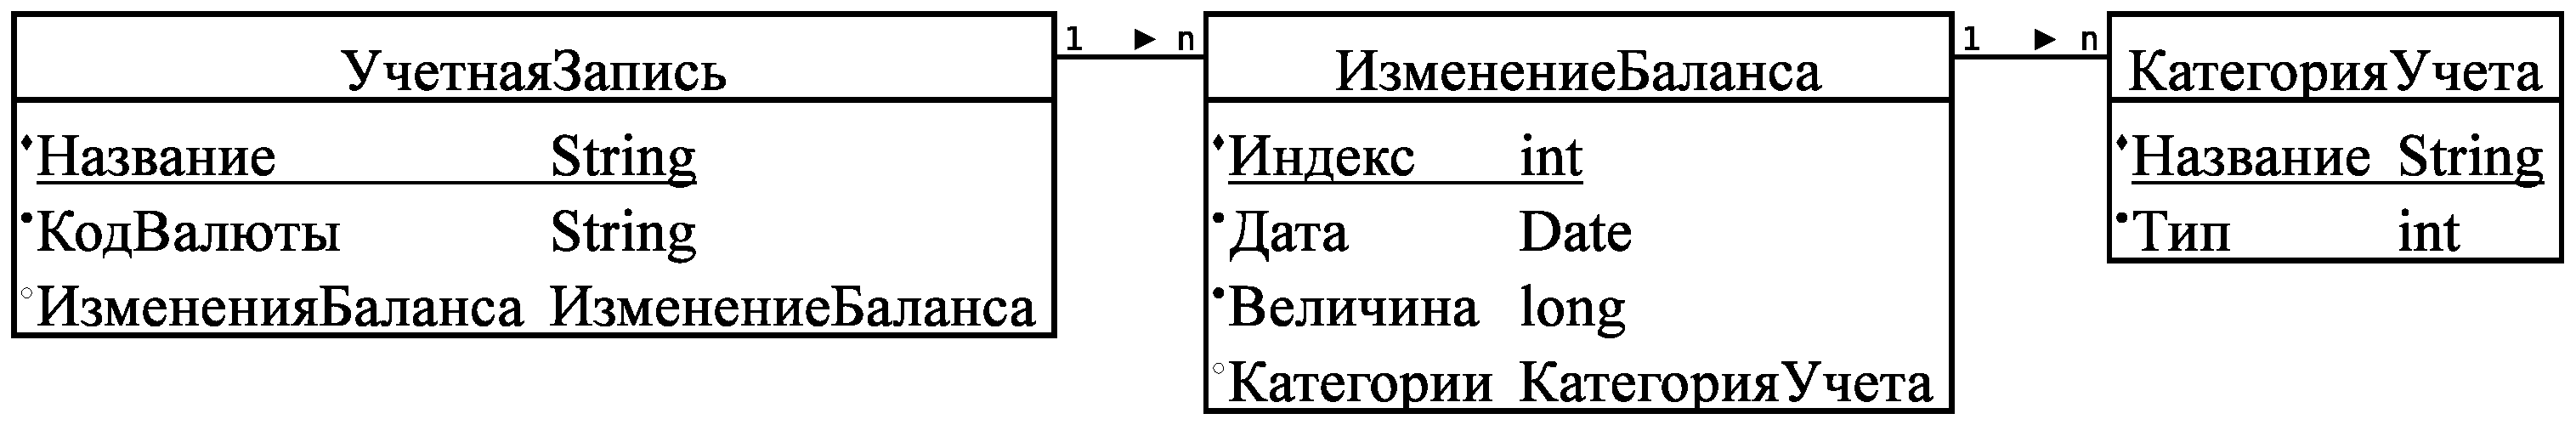
\includegraphics[width=140mm]{fig/design_entities.eps}
  }
  \caption{Модель данных приложения}
  \label{fig:design_entities}
\end{figure}

В соответствии с ней, сущность <<УчетнаяЗапись>> имеет поле названия,
являющееся ключевым, поле кода валюты, соответсвующее коду валюты
в соответствии со стандартом ISO 4217, а также ссылку на множество сущностей
<<ИзменениеБаланса>>. Данные сущности имеют служебное поле <<Индекс>>,
являющееся ключевым, поле даты регистрации, величины изменения баланса,
а также ссылку на множество связанных категорий.
Сущность <<Категория>> имеет ключевое поле названия, а также поле типа,
определяющее, относится ли данная категория к доходам или расходам.

Определенный интерес представляет вопрос выбора типа данных для хранения
значения изменения баланса. Дело в том, что для хранения финансовых данных
использовать дробные типы данных не рекомендуется
из-за ошибок округления~\cite{bloch08}. С другой стороны, не все СУБД
поддерживают специализированный тип данных для работы с валютой.
В связи с этим для хранения финансовой информации используется целочисленное
поле двойной длины (\textit{long}), младшие девять разрядов которого используются
для хранения дробной, а старшие --- для хранения целой части
исходной величины.

Ввод данных в приложение носит преимущественно ручной характер:
например, при вводе данных об изменении баланса
пользователь приложения должен ввести величину изменения баланса,
выбрать желаемые категории и указать дату.
Использование экспериментальной подсистемы компьютерного зрения
позволяет вводить данные о величине изменения баланса в
полуавтоматическом режиме.

Вывод данных производится в текстовом и графическом виде и
представляет как собственно хранимые данные, так и данные, полученные путем
применения агрегатных функций. Например, практический интерес представляют
суммы изменений баланса за указанный период, а также распределение
данных сумм по различным категориям учета.

% \subsection{Математическое обеспечение}

% Этапы процесса распознавания образов.
% Краткое математическое описание алгоримов, используемых на каждом этапе.
% Достоинства/недостатки/мотивация выбора.

% \subsection{Алгоритмическое обеспечение}

% % Проектирование алгоритма распознавания изображений.
% % Блок-схема окончательного алгоритма распознавания.

\subsection{Системные требования}

Разрабатываемое приложение предназначено для работы на мобильных устройствах
под управлением операционной системы Android версии не ниже 4.0.x (android-15).
Целевое устройство должно иметь ARM-совместимый процессор с тактовой частотой не менее
1 ГГц и располагать оперативной памятью объемом не менее 128 MБ.
Для полноценной работы приложения требуется наличие фотокамеры,
расположенной на тыльной стороне устройства.

\subsection{Эргономическое обеспечение}

В течение достаточно долгого времени внешний вид пользовательского интерфейса
приложений под управлением платформы Android не был регламентирован:
внешний вид, размещение и шаблоны взаимодействия различных элементов управления
были отданы на откуп разработчикам приложения.
Как следствие, внешний вид различных приложений мог заметно различаться.
Эта особенность представляла собой существенный недостаток платформы
с точки зрения пользователя.
В 2014 году компания Google представила сообществу Material Design ---
свод рекомендаций по оформлению элементов пользовательского интерфейса
мобильных приложений. Вместе с публикацией этих рекомендаций был
разработан набор библиотек, позволяющих реализовать их на предыдущих версиях платформы.
Данный свод рекомендаций находится в открытом доступе в сети
Интернет~\cite{material_design}.
В настоящее время подавляющее большинство приложений разрабатывается
в соответствии с ним.

Material design вводит ключевое понятие материала в контексте
пользовательского интерфейса приложения и рассматривает следующие
особенности его использования:
\begin{itemize}
\item общие рекомендации об эффективной организации интерфейса
  в виде паттернов поведения;
\item использование наборов цветов, иконок и шрифтов;
\item использование теней и отступов,
  а также анимации для переходов между различными состояниями.
\end{itemize}

Кроме этого, в нем приводится множество практических примеров
организации пользоваительского интерфейса.
На рисунке~\ref{fig:design_colors} представлена цветовая палитра
разрабатываемого приложения.

\begin{figure}[h!]
  \centering
  \fcolorbox{gray}{white}{
    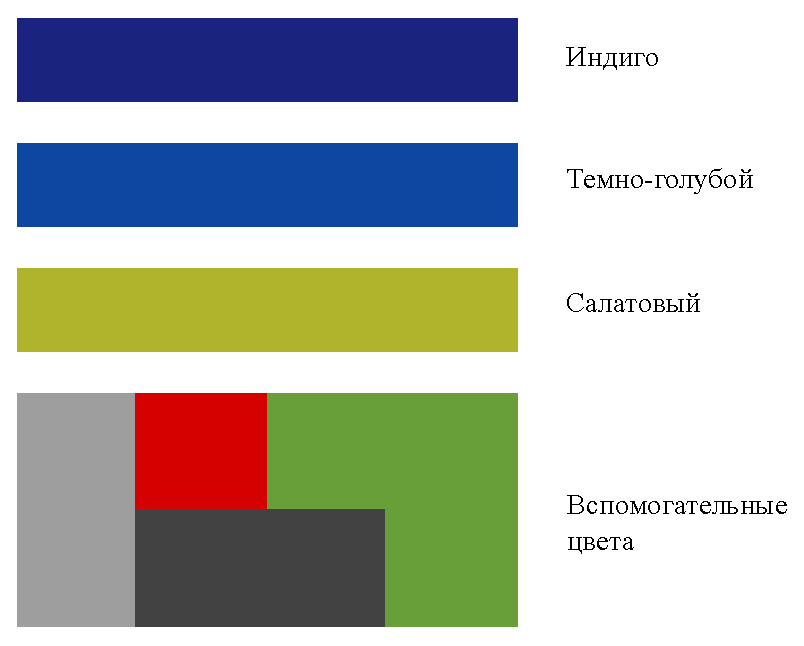
\includegraphics[width=140mm]{fig/design_colors.eps}
  }
  \caption{Используемая цветовая палитра}
  \label{fig:design_colors}
\end{figure}

Цвета <<индиго>> и <<темно-голубой>>
используются в качестве основных элементов интерфейса:
панели навигации, панелей выбора вкладок.
Салатовый цвет используется для подсвечивания выбранных вкладок,
а также выделения активных полей ввода.
Вспомогательные цвета используются в качестве фоновых цветов списков,
а также для оформления текста.

Material design предписывает использование семейства шрифтов
Roboto Sans для отображения текста, состоящего из латинских
и кириллических символов. Кроме этого, он регламентирует
использование различных размеров и начертаний данного шрифта.
Правилом хорошего тона является использование не более трех
различных начертаний шрифта на одном экране.
На рисунке~\ref{fig:design_fonts} приведен набор начертаний,
используемых в приложении.

\begin{figure}[h!]
  \centering
  \fcolorbox{gray}{white}{
    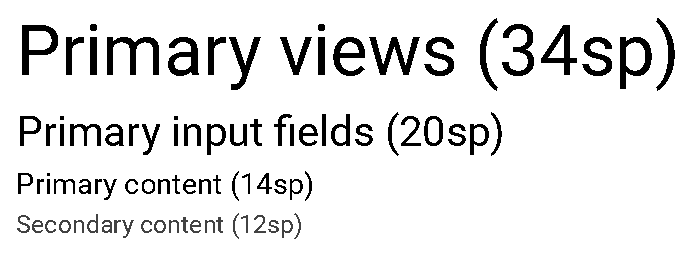
\includegraphics[width=140mm]{fig/design_fonts.eps}
  }
  \caption{Используемый набор начертаний}
  \label{fig:design_fonts}
\end{figure}

Все они основаны на базовом начертании шрифта Roboto Sans.
Размер начертаний указан в scale-independent pixels, учитывающих различия
в размерах и плотности дисплеев различных целевых устройств,
а также параметров настройки операционной системы.
Шрифт размером в 34sp применяется для отображения в первую очередь
текущего состояния счетов пользователя;
размер в 20sp используется при заполнении обязательных полей при вводе данных;
размеры 14sp и 12sp --- для отображения основного и вспомогательного текста
соответственно.

Кроме этого, разрабатываемое приложение использует иконки для
наглядного представления доступных пользователю опций меню.
Все они являются векторными изображениями, источником для них
является соответствующий репозиторий стандартных иконок.